\documentclass[webpdf,mynatbib,surname,nogrid,noCE,noMSC]{SYS}

\usepackage{cpl-oa}

\volname{}
\jvolume{0}
\jshort{syw}
\jvol{}
\jissue{0}
\cename{ES}

\mstype{Original article}

\pubyear{2016}
\copyyear{2016}
\artid{064}

\begin{document}

\title[T\"{O}PEL ET~AL.---SPECIESGEOCODER]{SpeciesGeoCoder: Fast Categorization of Species Occurrences for Analyses of Biodiversity, Biogeography, Ecology, and Evolution}

\author[]{M\textsc{ATS} \surname{T\textsc{\"{O}PEL}}$^{1,2,3,\ast}$, A\textsc{LEXANDER} \surname{Z\textsc{IZKA}}$^{3}$, M\textsc{ARIA} F\textsc{ERNANDA} \surname{C\textsc{ALI\'{O}}}$^{3,4,5}$, R\textsc{UUD} \surname{S\textsc{CHARN}}$^{3}$, D\textsc{ANIELE} \surname{S\textsc{ILVESTRO}}$^{3}$, \textsc{AND}~A\textsc{LEXANDRE} \surname{A\textsc{NTONELLI}}$^{3,6,\ast}$}

\address{$^{1}$Department of Marine Sciences, University of Gothenburg, PO Box 460, SE-405 30 G\"{o}teborg, Sweden; $^{2}$Bioinformatics Infrastructure for Life Sciences; $^{3}$Department of Biological and Environmental Sciences, University of Gothenburg, PO Box 461, SE-405 30 G\"{o}teborg, Sweden; $^{4}$Universidade de S\~{a}o Paulo, Instituto de Bioci\^{e}ncias, Departamento de Bot\^{a}nica, Rua do Mat\~{a}o, 277, Cidade Universit\'{a}ria, CEP: 05508-090, S\~{a}o Paulo, SP, Brazil; $^{5}$Universidade Estadual de Campinas, Instituto de Biologia, Departamento de Biologia Vegetal, Rua Monteiro Lobato, 255, Cidade Universit\'{a}ria, CEP: 13083-862, Campinas, SP, Brazil; $^{6}$Gothenburg Botanical Garden, Carl Skottsbergs gata 22A, SE-41319 G\"{o}teborg, Sweden;\\ $^{\ast}$Correspondence to be sent to: Bioinformatics infrastructure for Life Sciences, Department of Biological \& Environmental Sciences, University of Gothenburg, PO Box 463 SE-405 30 G�teborg, Sweden; E-mail: mats.topel@marine.gu.se; alexandre.antonelli@bioenv.gu.se.\\\vspace*{6pt} Mats T\"{o}pel and Alexander Zizka contributed equally to this article.}

\history{Received 2 December 2015; reviews returned 13 January 2016; accepted 8 July 2016}

\editor{Associate Editor: James Albert}

\abstract{Understanding the patterns and processes underlying the uneven distribution of biodiversity across space constitutes a major scientific challenge in systematic biology and biogeography, which largely relies on effectively mapping and making sense of rapidly increasing species occurrence data. There is thus an urgent need for making the process of coding species into spatial units faster, automated, transparent, and reproducible. Here we present SpeciesGeoCoder, an open-source software package written in Python and R, that allows for easy coding of species into user-defined operational units. These units may be of any size and be purely spatial (i.e., polygons) such as countries and states, conservation areas, biomes, islands, biodiversity hotspots, and areas of endemism, but may also include elevation ranges. This flexibility allows scoring species into complex categories, such as those encountered in topographically and ecologically heterogeneous landscapes. In addition, SpeciesGeoCoder can be used to facilitate sorting and cleaning of occurrence data obtained from online databases, and for testing the impact of incorrect identification of specimens on the spatial coding of species. The various outputs of SpeciesGeoCoder include quantitative biodiversity statistics, global and local distribution maps, and files that can be used directly in many phylogeny-based applications for ancestral range reconstruction, investigations of biome evolution, and other comparative methods.  Our simulations indicate that even datasets containing hundreds of millions of records can be analyzed in relatively short time using a standard computer. We exemplify the use of SpeciesGeoCoder by inferring the historical dispersal of birds across the Isthmus of Panama, showing that lowland species crossed the Isthmus about twice as frequently as montane species with a marked increase in the number of dispersals during the last 10 million years. [ancestral area reconstruction; biodiversity patterns; ecology; evolution; point in polygon; species distribution data.]}

\maketitle

Species distributions provide the basic knowledge for biodiversity research (\citealt{19Hortal2015}), including our understanding of species' environmental requirements, biogeographic history, and expected resilience to climate change. However, analyzing the distribution of the world's estimated 8.7 million species (\citealt{29Mora2011}) remains a major scientific challenge.

\begin{figure*}[!b]
\centerline{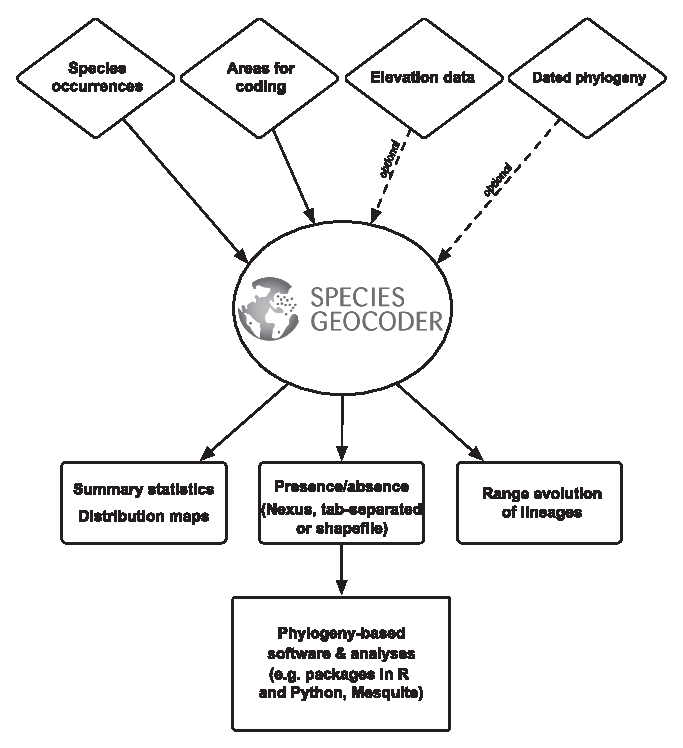
\includegraphics{OP-SYSB160066f1.eps}}
\caption{Simplified workflow of the SpeciesGeoCoder package. See text for details.}\label{f1}
\end{figure*}

There are now approximately 644 million species occurrences available through the Global Biodiversity Information Facility (GBIF; \href{http://www.gbif.org}{http://www.gbif.org}; accessed on April 21, 2016) and other biodiversity information networks, of which about 567 million are geo-referenced (provided with latitude and longitude data). These numbers include not only living species but also fossil taxa, allowing for biogeographic analyses based on both sources of data (e.g., \citealt{3Antonelli2015}; \citealt{37Silvestro2016}). Species occurrence data are steadily increasing thanks to new agreements on data sharing, on-going digitalization programs, and tools that enable automated geo-referencing of older museum specimens (\citealt{16Guralnick2006}; \citealt{14Garcia-Milagros2010}).

Publicly available species occurrences represent an enormous data source for biodiversity research, but are as yet poorly exploited due to two main factors: (i) general skepticism concerning the quality of records available, in terms of species identification and precise coordinates (\citealt{34Robertson2016}; Antonelli in press); and (ii) demonstrated taxonomic, geographic, and temporal biases (\citealt{8Boakes2010}; \citealt{26Meyer2015}). Improving quality relies on data curation---practiced by some country-level projects such as Flora Hellenica (\citealt{39Strid2000})---as well as tools for automated data cleaning, for example through workflows such as the Biodiversity Virtual e-Laboratory (\citealt{40Vicario2011}) and packages such as ``biogeo'' (\citealt{34Robertson2016}). Finally, taxonomic misidentifications may be common (\citealt{15Goodwin2015}), which may lead to erroneous inferences on the total distribution of a species. While an empirical assessment of the accuracy of each observation cannot be easily automated, it should be possible to assess the influence of random identification errors on the geographic ranges of species.

To make sense of biological distributions, raw species occurrences often need to be classified into discrete categories. These can then be used in connection with a phylogeny for historical biogeographic analyses including ancestral range reconstructions (\citealt{33Ree2008}; \citealt{21Landis2013}; \citealt{24Matzke2013}) and area-dependent inferences of diversification rates (\citealt{36Silvestro2011}; \citealt{13FitzJohn2012}). Species categorization into commonly recognized areas such as eco-regions and realms (\citealt{31Olson2001}; \citealt{1Abell2008}; \citealt{18Holt2013}) and biogeographic regions or bioregions (\citealt{41Vilhena2015}; Edler et~al. this issue) may reveal patterns of biodiversity and distribution at a large scale, facilitating the identification of regions with outstanding levels of species richness and endemism that is central to the concept of biodiversity hotspots (\citealt{30Myers2000}). Rapidly increasing species occurrence data and the need to classify species into discrete areas in an automated, reproducible, and transparent way has led us to develop SpeciesGeoCoder.

\section*{D{\sc ESCRIPTION}}

The source code consists of a set of python modules, centered on a point-in-polygon algorithm that determines if a species locality record is found inside or outside of a particular polygon. The analysis of geoTIFF files is done using the GDAL python bindings (\href{http://www.gdal.org/}{http://www.gdal.org/}) for fast execution. The basic workflow is illustrated in Figure~\ref{f1} and described below:
\begin{enumerate}
\item[1.] The user provides two files. The first should contain species occurrence data, including species names, latitude, and longitude in either (i) tab-separated format, (ii) the CSV format provided by \href{http://www.gbif.org}{www.gbif.org}, or (iii) in shapefile format. The second file defines the areas of interest in tab-separated format (i.e., a list of named polygons, and---optionally---an elevation or sea depth range such as between 1000 and 2000~m a.s.l., or between 0 and $-$30~m) or as a shapefile. Polygon files can be generated easily with various GIS tools, and a tutorial is available at https://github.com/mtop/speciesgeocoder/wiki for the freely available program QGIS (\href{http://qgis.osgeo.org}{http://qgis.osgeo.org}). If an elevation range is provided for the polygons, then elevation data in the form of geotiff files is also required, and these can be downloaded from various online resources (see the wiki for tutorials, links, and example files); 
\item[2.] SpeciesGeoCoder loops through the input file and counts the number of occurrences of each species in each polygon, and optionally takes the elevation constraints into account; 
\item[3.] The default output format is a Nexus file containing a data matrix with all analyzed species and their presence (1) or absence (0) in each area. ``Presence'' requires by default at least one occurrence in an area, but user-defined thresholds may be set instead. This means that outlier localities incorrectly assigned to a polygon (e.g., due to an erroneous shift between latitude and longitude) can be easily identified. Alternatively, the user may request a more complex output including the number of occurrences in each polygon, which could further aid the identification of outliers. The Nexus file can then be analyzed in programs such as Mesquite (\citealt{22Maddison2009}) and most phylogenetic packages written in R, such as APE (\citealt{32Paradis2004}), geiger (\citealt{17Harmon2008}), Diversitree (\citealt{13FitzJohn2012}), BayArea (\citealt{21Landis2013}), and BioGeoBEARS (\citealt{25Matzke2014}), as well as others written in Python, such as BayesRate (\citealt{36Silvestro2011}), and Biopython (\citealt{10Cock2009}). SpeciesGeoCoder can also export the result of an analysis in tab-separated text format for easy parsing and additional analyses.  Localities identified inside any of the polygons analyzed can also be exported in shapefile format, which gives a convenient way of extracting a subset of localities from a larger data set; 
\item[4.] The second (optional) type of output is a series of summary statistics and distribution maps.  These include multiple pdf documents with bar charts as graphical representations of the number of species per area, the number of occurrences per species per area, and the relative occurrence per area for each species. The summary tables used for the graphical output are also made available as tab-separated text files. The distribution maps plot all occurrence points and the areas included in the analyses. In addition, for small data sets comprising less than 40 species, a coexistence matrix for each area is calculated and visualized as a heat map. These files help not only with biological interpretations, but also to identify problematic occurrence points that need further verification; 
\item[5.] The third (optional) output is a series of plots summarizing the historical dispersal of lineages between all pairs of user-defined areas, based on one or a sample of dated phylogenies.  These plots are generated with R scripts, using by default stochastic mapping to infer shifts in transitions along branches, and the computation of absolute as well as relative (i.e., corrected by the number of lineages) number of dispersals through time (\citealt{35Silvestro2012}; \citealt{12Fernandez-Mendoza2013}; \citealt{3Antonelli2015}); 
\item[6.] The fourth (optional) output includes a sensitivity test aimed at quantifying the potential effects of incorrectly identified specimens in the input data on the coded geographic ranges. In this test, we assume that each geo-referenced occurrence has a probability $r$~to be misidentified. An occurrence mistakenly assigned to a species should be removed from the data when coding the species distribution. However, its removal may or may not change the geographic distribution of the species coded within discrete areas depending on whether other (correctly identified) occurrences of the species are found in the same geographic unit. In our sensitivity test, occurrences that are randomly selected as misidentified are removed from the data and the geographic distribution of the species is re-coded based on the sub-sampled occurrences. This procedure is repeated for all occurrences 10,000 times under error probabilities equal to 0.05, 0.10, 0.25, and 0.50. The results of these tests are summarized in terms of average number of species in a data set that change in their coded range under different scenarios of errors, compared to their ranges estimated from all occurrence data. Additionally, we compute the probability that a random error affects the coded distribution of each species and provide these probabilities for each species in a data set (thereby identifying which species are most sensitive to error given the number of occurrences and their distribution under different error probabilities). These results are saved in tab-separated tables.
\end{enumerate}
\noindent The overall design of SpeciesGeoCoder is done with extensibility in mind. The package is composed of a set of python classes for storing and manipulating locality and polygon data in different input formats, so users with experience in object-oriented programing should be able to extend the package with additional features or contact the authors for proposing novel implementations.

\begin{figure*}[!b]
\centerline{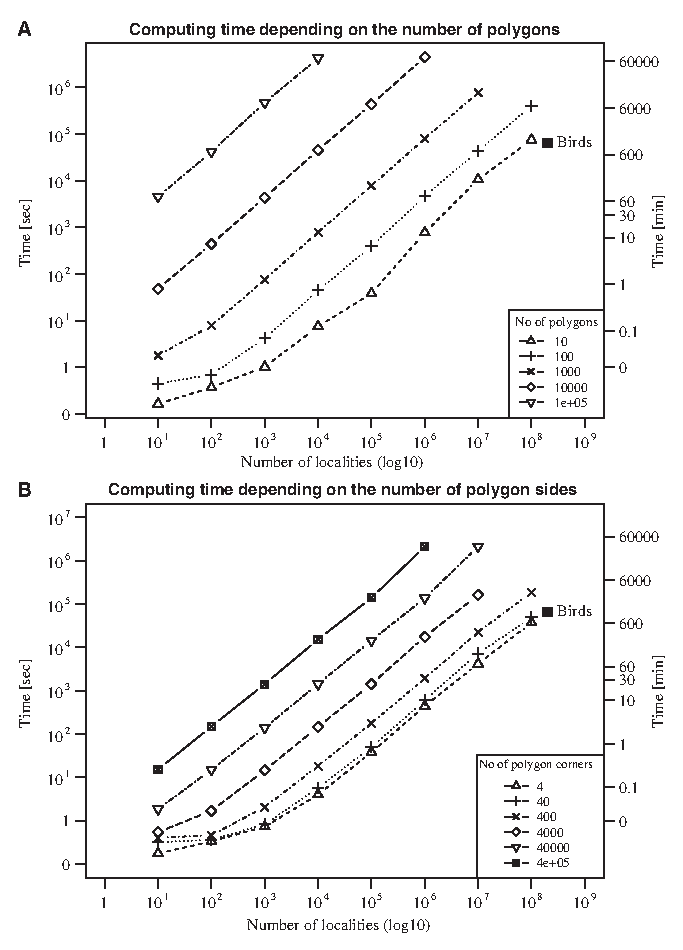
\includegraphics{OP-SYSB160066f2.eps}}
\caption{Computational time in relation to the increase in A) number of polygons and B) polygon complexity (number of polygon corners) and number of species occurrences. As a comparison to empirical data, the square labeled ``Birds'' corresponds to the coding of approximately 200,000,000 bird occurrences available from ebird.org. The analyses were performed on a standard computer with a 1.9 MHz processor.}\label{f2}
\end{figure*}

\section*{B{\sc ENCHMARK}}

We tested the performance and scalability of our package through a series of simulations on a five-year-old computer with four 12-core 1.9 MHz AMD Opteron 6168 processors. All benchmarks, except the ones examining multiprocessor performance, were ran on one CPU and we focused on how computing time was determined by three key variables: (i)the number of geo-referenced occurrences, (ii) the number of polygons, and (iii) the complexity of the polygons, measured by their number of corners (i.e., vertices or nodes). An occurrence dataset (i) was simulated as a set of globally distributed localities (see example in Supplementary Fig. S1 in Supplementary Material). The polygon dataset (ii) was generated in a similar way, by creating a grid of square polygons sharing two corners with each of its neighboring polygons (Supplementary Fig. S2 in Supplementary Material). The polygon complexity dataset (iii) was generated by creating one square polygon, and successively adding nodes equally distributed over its perimeter (Supplementary Fig. S3 in Supplementary Material). This approach of generating polygons with an increasing number of coordinate pairs (i.e., nodes) is suitable for benchmarking purposes since the computation time for the point-in-polygon algorithm implemented in SpeciesGeoCoder is not affected by the actual shape of the polygon, but only by the number of coordinates that make up the polygon. The simulations were then performed with a logarithmical increase in the number of occurrences, polygons, and polygon nodes, ranging between 10$^{1}$ and 10$^{8}$.

Our\enlargethispage{3pt} results (Fig.~\ref{f2}) show that there is a nearly linear relationship between the computation time required and (i) the number of localities, (ii) the number of polygons, and (iii) the complexity of the polygons analyzed. Doubling the amount of input data will also double the analysis time. In addition, we examined how well the parallelization of the code worked by running analyses on 10 million localities and 100 polygons using 1, 2, 4, 8, 16 and 32 CPUs. We found a negative linear correlation between the computation time and the number of CPUs utilized, and that doubling the number of CPUs will decrease the computation time with nearly 50{\%}. These results lead us to the conclusion that SpeciesGeoCoder can handle vast amounts of data---millions of polygons and occurrences---within feasible time using standard computers.

\begin{figure*}[!b]
\centerline{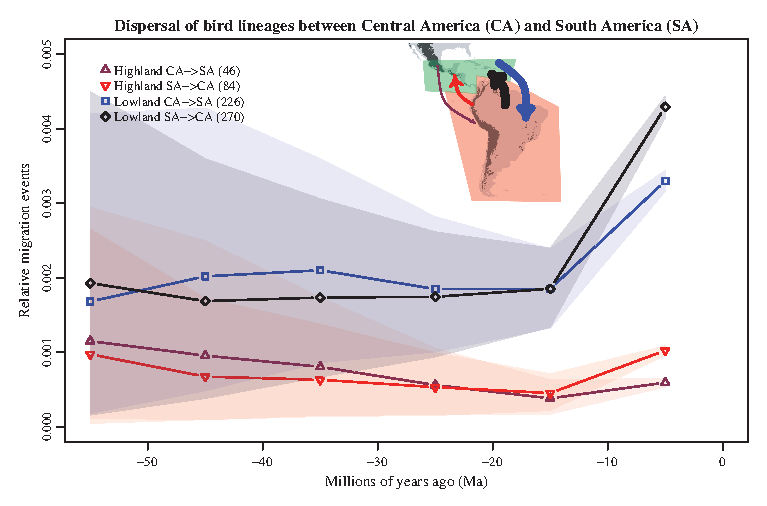
\includegraphics{OP-SYSB160066f3.eps}}
\caption{Historical dispersal of lowland and highland bird lineages between South America (SA) and Central America (CA), calculated per 10-million-year time bins. The total number of dispersal events inferred for our data set is indicated between brackets in the legend. The inset shows the two polygons used for coding all bird species, with arrows colored as in the curves for migration events and their width proportional to the total number of events.} \label{f3}
\end{figure*}

\section*{B{\sc IOLOGICAL} E{\sc XAMPLE}}

We\enlargethispage{3pt} inferred the historical dispersal of montane and lowland bird lineages through time across the Central American Seaway, which separated North and South America for millions of years until the emergence of the Isthmus of Panama (\citealt{5Bacon2015a}, \citeyear{6Bacon2015b}; \citealt{28Montes2015}). First, we downloaded the full occurrence data set for all birds including approximately 10,000 species and 200,000,000 records from \href{http://www.ebird.org}{http://www.ebird.org} (eBird 2013). We then used SpeciesGeoCoder to exclude all records found outside the South American continent, as well as all those found north of the Tropic of Cancer, and coded the remaining species into Central America and South America.  We defined the border between South and Central America following the Uramita fault (\citealt{27Montes2012}) that separates the South American and the Panamanian geological plates (Fig.~\ref{f3}). We created two operational units from each polygon, one including occurrences below 1000 m a.s.l. (lowlands) and the second including occurrences above 1000 m a.s.l.  (highlands) following the same categorization as \citet{42Weir2006}. We then reconstructed ancestral areas onto the species-level dated phylogeny of birds provided by \citet{20Jetz2012}, using stochastic mapping to reconstruct the historical dispersal of lineages through time among these four operational units. We calculated both the total (absolute) as well as the relative (in proportion to the number of lineages) number of dispersals between each pair of areas, using bins of 10 million years. Since not all bird species could be matched between the phylogeny and the occurrence data set, the final analyses included 4350 species.

We tested the sensitivity of the geographic categorization of bird species to identification errors using the procedure described above. A random error equal to 5{\%} would affect the coded geographic distribution of 48 ($\pm 11$) species (${\sim}1{\%}$ of the dataset), whereas a 10{\%} error frequency would affect 79 ($\pm 14$) species (${\sim}2{\%}$). Only a very high error frequency of 50{\%} (where one in two samples would be wrongly identified to species level) would affect more than 5{\%} of the species in our dataset ($250 \pm 25$ species), thus indicating that area categorization in this case is robust to random identification errors. Detailed output of the sensitivity test is provided in Supplementary Table S1 in Supplementary Material (available at Dryad at \href{http://dx.doi.org/10.5061/dryad.tm32k}{http://dx.doi.org/10.5061/dryad.tm32k}).

Although the variation among reconstructions is large, our results suggest that dispersals between the lowlands of South and Central America occurred consistently more frequently (c. 2--4 times) than dispersals between the highlands of those landmasses (Supplementary Figures S3 and S4 in Supplementary Material). There were no major differences in directionality of dispersals, except for the last time bin considered (0--10~Ma) when northward dispersals dominated. This supports the conclusion by \citet{43Weir2009} that birds mainly followed an opposite route during the Great American Biotic Interchange as compared with mammals, which migrated mostly southwards and in more recent times (\citealt{38Stehli1985}; \citealt{9Carrillo2014}; \citealt{4Bacon2016}). The rate of dispersals increased for all categories in the last time bin, probably as a consequence of the emergence of the Panama Isthmus in the last 13~Ma (\citealt{5Bacon2015a}, \citeyear{6Bacon2015b}; \citealt{28Montes2015}). Dispersals in previous time periods seem to follow a rather uniform, stochastic rate (de Baets et~al. in press) that is also reflected by sporadic fossil findings such as a recently described South American primate in the early Miocene (20.9~Ma) of Panama (\citealt{7Bloch2016}).\vs{-6}

\section*{C{\sc ONCLUSIONS}}

We have shown that SpeciesGeoCoder allows for easy and fast categorization of species distribution data for various analyses in biogeography, ecology, and evolution. Beyond the example provided here, the output obtained could be readily used for calculating measures of alpha, beta, and gamma diversity; the identification of neglected areas for conservation; and providing real-time detection of GPS-tagged animals entering and leaving protected areas. Finally, the visualization and coding of species into areas may greatly facilitate cleaning up occurrence databases, by enabling the identification of outliers that may require additional examination or exclusion from subsequent analyses (\citealt{23Maldonado2015}).

Although several of the functions in SpeciesGeoCoder could be performed in other software by an advanced GIS user, our package offers a number of advantages: it is fast, increases reproducibility of analyses, allows exploration of alternative sets of polygons for area coding, can handle large files, is particularly suitable for phylogenetic and biogeographic analyses, enables the inclusion of thresholds for coding, assesses the effect of misidentified specimens, includes elevation or depth, allows for batch processing, is directly integrated with stochastic mapping, produces summary tables and maps, among others. We therefore hope that SpeciesGeoCoder will become an indispensible tool for coding species into discrete units, as is required for most currently available parametric methods in historical biogeography and for the exploration of biodiversity patterns.\vs{-6}

\section*{A{\sc VAILABILITY}}

SpeciesGeoCoder is available for download from \href{https://github.com/mtop/speciesgeocoder/releases}{https://github.com/mtop/speciesgeocoder/releases}.  The current release includes installation instructions for Mac OSX, Gnu/Linux, and Windows; example files, tutorials, plug-in scripts, and useful links. The program with complementary functions is also available for the R environment (speciesgeocodeR) from CRAN at \href{http://cran.r-project.org/web/packages/speciesgeocodeR/index.html}{https://cran.r-project.org/web/packages/}\break \href{http://cran.r-project.org/web/packages/speciesgeocodeR/index.html}{speciesgeocodeR/index.html}, as well as via a web interface at \href{http://portal.bils.se/speciesgeocoder/tool}{https://portal.bils.se/speciesgeocoder/}\break \href{http://portal.bils.se/speciesgeocoder/tool}{tool}. Links to all resources are available at \href{http://github.com/mtop/speciesgeocoder/wiki}{https://github.com/mtop/speciesgeocoder/wiki}, \href{http://github.com/azizka/speciesgeocodeR/wiki}{https://github.com/azizka/speciesgeocodeR/wiki} or from \href{http://antonelli-lab.net}{http://antonelli-lab.net}.\vs{-6}

\section*{S{\sc UPPLEMENTARY} M{\sc ATERIAL}}

Supplementary material, including data files and online-only appendices, can be found in the Dryad data repository at \href{http://dx.doi.org/10.5061/dryad.tm32k}{http://dx.doi.org/10.5061/dryad.tm32k}.\vs{-6}

\section*{F{\sc UNDING}}

Funding was provided by the Swedish Research Council (B0569601), the European Research Council under the European Union's Seventh Framework Programme (FP/2007-2013, ERC Grant Agreement no.  331024), and a Wallenberg Academy Fellowship to A.A.; from Carl Tryggers stiftelse (CTS 11:479, CTS 12:507) to M.T.; and from Funda\c{c}\~{a}o de Amparo \`{a} Pesquisa do Estado de S\~{a}o Paulo (FAPESP 2009/52161-2, 2013/10262-2) to M.F.C.\vs{-6}

\section*{A{\sc CKNOWLEDGMENTS}}

We thank Rosemeri Morokawa, Alexander Walther, students and colleagues at our research groups for fruitful discussions and software testing; Paula T\"{o}pel for designing the SpeciesGeoCoder logo; Johan Viklund and the Bioinformatics Infrastructure for Life Sciences (\href{https://bils.se/}{https://bils.se/}) for implementing the web interface. The code was developed, tested, and benchmarked on the bioinformatics computer cluster Albiorix (http://albiorix.bioenv.gu.se/) at the Department of Biological and Environmental Sciences, University of Gothenburg. Author contributions: A.A. and M.T. conceived the original idea and initiated the project, with subsequent contributions from all authors; M.T. wrote the Python code; A.Z. and D.S. contributed the R functionalities; M.F.C., M.T., and R.S. performed the benchmarking; M.F.C. and R.S. wrote the QGIS tutorial; M.F.C., A.Z., R.S., D.S., and M.T. analyzed the data; A.A. and M.T. led the writing with substantial contributions from all authors.

\begin{thebibliography}{}

\bibitem[Abell et~al.(2008)Abell Thieme Revenga Bryer Kottelat Bogutskaya Coad Mandrak Balderas Bussing ]{1Abell2008} Abell R., Thieme M.L., Revenga C., Bryer M., Kottelat M., Bogutskaya N., Coad B., Mandrak N., Balderas S.C., Bussing W. 2008. Freshwater ecoregions of the world: a new map of biogeographic units for freshwater biodiversity conservation. Bioscience 58:403--414.

\bibitem[Antonelli(Forthcoming)Antonelli ]{2AntonelliForthcoming} Antonelli A. Forthcoming. Advancing biodiversity research: comparative biogeography, big data, and common myths. Scientia Danica.

\bibitem[Antonelli et~al.(2015)Antonelli Zizka Silvestro Scharn Cascales-Mi\~{n}ana Bacon ]{3Antonelli2015} Antonelli A., Zizka A., Silvestro D., Scharn R., Cascales-Mi\~{n}ana B., Bacon C.D. 2015. An engine for global plant diversity: highest evolutionary turnover and emigration in the American tropics. Front. Genet. 6:130.

\bibitem[Bacon et~al.(2016)Bacon Molnar Antonelli Crawford Montes Vallejo-Pareja ]{4Bacon2016} Bacon C.D., Molnar P., Antonelli A., Crawford A.J., Montes C., Vallejo-Pareja M.C. 2016.  Quaternary glaciation and the Great American Biotic Interchange. Geology 10.1130/G37624.1.

\bibitem[Bacon et~al.(2015a)Bacon Silvestro Jaramillo Smith Chakrabarty Antonelli ]{5Bacon2015a} Bacon C.D., Silvestro D., Jaramillo C., Smith B.T., Chakrabarty P., Antonelli A. 2015a. Biological evidence supports an early and complex emergence of the Isthmus of Panama. Proc. Natl. Acad. Sci.  USA 112:6110--6115.

\bibitem[Bacon et~al.(2015b)Bacon Silvestro Jaramillo Smith Chakrabarty Antonelli ]{6Bacon2015b} Bacon C.D., Silvestro D., Jaramillo C., Smith B.T., Chakrabarty P., Antonelli A. 2015b. Reply to Lessios and Marko et~al.: early and progressive migration across the Isthmus of Panama is robust to missing data and biases. Proc. Natl. Acad. Sci. USA 112:E5767--E5768.

\bibitem[Bloch et~al.(2016)Bloch Woodruff Wood Rincon Harrington Morgan Foster Montes Jaramillo Jud$,$ Jones MacFadden ]{7Bloch2016} Bloch J.I., Woodruff E.D., Wood A.R., Rincon A.F., Harrington A.R., Morgan G.S., Foster D.A., Montes C., Jaramillo C.A., Jud N.A.$,$ Jones D.S., MacFadden B.J. 2016. First North American fossil monkey and early Miocene tropical biotic interchange. Nature, advance online publication doi: 10.1038/nature17415.

\bibitem[Boakes et~al.(2010)Boakes McGowan Fuller Chang-qing Clark O'Connor Mace ]{8Boakes2010} Boakes E.H., McGowan P.J., Fuller R.A., Chang-qing D., Clark N.E., O'Connor K., Mace G.M. 2010.  Distorted views of biodiversity: spatial and temporal bias in species occurrence data. PLoS Biol.  8:e1000385.

\bibitem[Carrillo et~al.(2014)Carrillo Forasiepi Jaramillo S\'{a}nchez-Villagra ]{9Carrillo2014} Carrillo J.D., Forasiepi A., Jaramillo C., S\'{a}nchez-Villagra M.R. 2014. Neotropical mammal diversity and the Great American Biotic Interchange: spatial and temporal variation in South America's fossil record. Front. Genet. 5:451.

\bibitem[Cock et~al.(2009)Cock Antao Chang Chapman Cox Dalke Friedberg Hamelryck Kauff Wilczynski ]{10Cock2009} Cock P.J., Antao T., Chang J.T., Chapman B.A., Cox C.J., Dalke A., Friedberg I., Hamelryck T., Kauff F., Wilczynski B. 2009. Biopython: freely available Python tools for computational molecular biology and bioinformatics. Bioinformatics 25:1422--1423.

\bibitem[de Baets et~al.(2016)de Baets Antonelli Donoghue ]{11deForthcoming} de Baets K., Antonelli A., Donoghue P.C.J. 2016. Tectonic blocks and molecular clocks. Philos.  Trans. R. Soc. Ser. B Biol. Sci. 371(1699):201060098.

\bibitem[Fern\'{a}ndez-Mendoza and Printzen(2013)Fern\'{a}ndez-Mendoza Printzen ]{12Fernandez-Mendoza2013} Fern\'{a}ndez-Mendoza F., Printzen C. 2013. Pleistocene expansion of the bipolar lichen Cetraria aculeata into the Southern hemisphere. Mol. Ecol. 22:1961--1983.

\bibitem[FitzJohn(2012)FitzJohn ]{13FitzJohn2012} FitzJohn R.G. 2012. Diversitree: comparative phylogenetic analyses of diversification in R.  Methods Ecol. Evol. 3:1084--1092.

\bibitem[Garcia-Milagros and Funk(2010)Garcia-Milagros Funk ]{14Garcia-Milagros2010} Garcia-Milagros E., Funk V.A. 2010. Improving the use of information from museum specimens: using Google Earth\copyright to georeference Guiana Shield specimens in the US National Herbarium.  Front. Biogeogr. 2:71--77.

\bibitem[Goodwin et~al.(2015)Goodwin Harris Filer Wood Scotland ]{15Goodwin2015} Goodwin Z.A., Harris D.J., Filer D., Wood J.R.I., Scotland R.W. 2015. Widespread mistaken identity in tropical plant collections. Curr. Biol. 25:R1066--R1067.

\bibitem[Guralnick et~al.(2006)Guralnick Wieczorek Beaman Hijmans the BioGeomancer Working Group]{16Guralnick2006} Guralnick R.P., Wieczorek J., Beaman R., Hijmans R.J., the BioGeomancer Working Group. 2006.  BioGeomancer: automated Georeferencing to Map the World's Biodiversity Data. PLoS Biol. 4:e381.

\bibitem[Harmon et~al.(2008)Harmon Weir Brock Glor Challenger ]{17Harmon2008} Harmon L.J., Weir J.T., Brock C.D., Glor R.E., Challenger W. 2008. GEIGER: investigating evolutionary radiations. Bioinformatics 24:129--131.

\bibitem[Holt et~al.(2013)Holt Lessard Borregaard Fritz Ara\'{u}jo Dimitrov Fabre Graham Graves J{\o}nsson ]{18Holt2013} Holt B.G., Lessard J.-P., Borregaard M.K., Fritz S.A., Ara\'{u}jo M.B., Dimitrov D., Fabre P.-H., Graham C.H., Graves G.R., J{\o}nsson K.A. 2013. An update of Wallace's zoogeographic regions of the world. Science 339:74--78.

\bibitem[Hortal et~al.(2015)Hortal de Bello Diniz-Filho Lewinsohn Lobo Ladle ]{19Hortal2015} Hortal J., de Bello F., Diniz-Filho J.A.F., Lewinsohn T.M., Lobo J.M., Ladle R.J. 2015. Seven shortfalls that beset large-scale knowledge on biodiversity. Annu. Rev. Ecol. Syst. 46:523--549.

\bibitem[Jetz et~al.(2012)Jetz Thomas Joy Hartmann Mooers ]{20Jetz2012} Jetz W., Thomas G., Joy J., Hartmann K., Mooers A. 2012. The global diversity of birds in space and time. Nature 491:444--448.

\bibitem[Landis et~al.(2013)Landis Matzke Moore Huelsenbeck ]{21Landis2013} Landis M.J., Matzke N.J., Moore B.R., Huelsenbeck J.P. 2013. Bayesian analysis of biogeography when the number of areas is large. Syst. Biol. 62:789--804.

\bibitem[Maddison and Maddison(2009)Maddison Maddison ]{22Maddison2009} Maddison W.P., Maddison D.R. 2009. Mesquite: a modular system for evolutionary analysis. Version 2.71 http://mesquiteproject.org.

\bibitem[Maldonado et~al.(2015)Maldonado Molina Zizka Persson Taylor Alb\'{a}n Chilquillo R{\o}nsted Antonelli ]{23Maldonado2015} Maldonado C., Molina C.I., Zizka A., Persson C., Taylor C.M., Alb\'{a}n J., Chilquillo E., R{\o}nsted N., Antonelli A. 2015. Estimating species diversity and distribution in the era of Big Data: to what extent can we trust public databases? Global Ecol. Biogeogr. 24:973--984.\vpb{}

\bibitem[Matzke(2013)Matzke ]{24Matzke2013} Matzke N.J. 2013. BioGeoBEARS: BioGeography with Bayesian (and Likelihood) Evolutionary Analysis in R Scripts. Berkeley (CA): University of California, Berkeley.

\bibitem[Matzke(2014)Matzke ]{25Matzke2014} Matzke N.J. 2014. Model selection in historical biogeography reveals that founder-event speciation is a crucial process in Island Clades. Syst. Biol. 63:951--970.

\bibitem[Meyer et~al.(2015)Meyer Kreft Weigelt ]{26Meyer2015} Meyer C., Kreft H., Weigelt P. 2015. Multidimensional biases, gaps and uncertainties in global plant occurrence information. PeerJ PrePrints 3:e1635.

\bibitem[Montes et~al.(2012)Montes Bayona Cardona Buchs Silva Mor\'{o}n Hoyos Ram\'{\i}rez Jaramillo Valencia ]{27Montes2012} Montes C., Bayona G., Cardona A., Buchs D.M., Silva C.A., Mor\'{o}n S., Hoyos N., Ram\'{\i}rez D.A., Jaramillo C.A., Valencia V. 2012. Arc-continent collision and orocline formation: closing of the Central American seaway. J. Geophys. Res. 117:B04105.

\bibitem[Montes et~al.(2015)Montes Cardona Jaramillo Pardo Silva Valencia Ayala P\'{e}rez-Angel Rodriguez-Parra Ramirez Ni\~{n}o ]{28Montes2015} Montes C., Cardona A., Jaramillo C., Pardo A., Silva J.C., Valencia V., Ayala C., P\'{e}rez-Angel L.C., Rodriguez-Parra L.A., Ramirez V., Ni\~{n}o H. 2015. Middle Miocene closure of the Central American Seaway. Science 348:226--229.

\bibitem[Mora et~al.(2011)Mora Tittensor Adl Simpson Worm ]{29Mora2011} Mora C., Tittensor D.P., Adl S., Simpson A.G.B., Worm B. 2011. How many species are there on earth and in the ocean? PLoS Biol. 9:e1001127.

\bibitem[Myers et~al.(2000)Myers Mittermeler Mittermeler Da Fonseca Kent ]{30Myers2000} Myers N., Mittermeler R.A., Mittermeler C.G., Da Fonseca G.A.B., Kent J. 2000. Biodiversity hotspots for conservation priorities. Nature 403:853--858.

\bibitem[Olson et~al.(2001)Olson Dinerstein Wikramanayake Burgess Powell Underwood D'amico Itoua Strand Morrison ]{31Olson2001} Olson D.M., Dinerstein E., Wikramanayake E.D., Burgess N.D., Powell G.V., Underwood E.C., D'amico J.A., Itoua I., Strand H.E., Morrison J.C. 2001. Terrestrial ecoregions of the world: a new map of life on earth. Bioscience 51:933--938.

\bibitem[Paradis et~al.(2004)Paradis Claude Strimmer ]{32Paradis2004} Paradis E., Claude J., Strimmer K. 2004. APE: Analyses of Phylogenetics and Evolution in R language. Bioinformatics 20:289--290.

\bibitem[Ree and Smith(2008)Ree Smith ]{33Ree2008} Ree R.H., Smith S.A. 2008. Maximum likelihood inference of geographic range evolution by dispersal, local extinction, and cladogenesis. Syst. Biol. 57:4--14.

\bibitem[Robertson et~al.(2016)Robertson Visser Hui ]{34Robertson2016} Robertson M.P., Visser V., Hui C. 2016. Biogeo: an R package for assessing and improving data quality of occurrence record datasets. Ecography 39:394--401.

\bibitem[Silvestro(2012)Silvestro ]{35Silvestro2012} Silvestro D. 2012. Diversification in time and space. Methodological advancement and case studies from the Neotropical plant family Bromeliaceae. Frankfurt am Main, Germany: Johann-Wolfgang-Goethe-University.

\bibitem[Silvestro et~al.(2011)Silvestro Schnitzler Zizka ]{36Silvestro2011} Silvestro D., Schnitzler J., Zizka G. 2011. A Bayesian framework to estimate diversification rates and their variation through time and space. BMC Evol. Biol. 11:311.

\bibitem[Silvestro et~al.(2016)Silvestro Zizka Bacon Cascales-Mi\~{n}ana Salamin Antonelli ]{37Silvestro2016} Silvestro D., Zizka A., Bacon C.D., Cascales-Mi\~{n}ana B., Salamin N., Antonelli A. 2016. Fossil Biogeography: a new model to infer dispersal, extinction and sampling from paleontological data.  Philos. Trans. R. Soc. B doi:~10.1098/rstb.2015.0225

\bibitem[Stehli and Webb(1985)Stehli Webb ]{38Stehli1985} Stehli F.G., Webb S.D. 1985. The Great American biotic interchange. New York, London: Plenum Press.

\bibitem[Strid(2000)Strid ]{39Strid2000} Strid A. 2000. The Flora Hellenica database. Portugaliae Acta Biologica 19:49--59.

\bibitem[Vicario et~al.(2011)Vicario Hardisty Haitas ]{40Vicario2011} Vicario S., Hardisty A., Haitas N. 2011. Biovel: biodiversity virtual e-laboratory. EMBnet. J.  17:5--6.

\bibitem[Vilhena and Antonelli(2015)Vilhena Antonelli ]{41Vilhena2015} Vilhena D.A., Antonelli A. 2015. A network approach for identifying and delimiting biogeographical regions. Nat. Commun. 6:6848.

\bibitem[Weir(2006)Weir ]{42Weir2006} Weir J.T. 2006. Divergent timing and patterns of species accumulation in lowland and highland neotropical birds. Evolution 60:842--855.

\bibitem[Weir et~al.(2009)Weir Bermingham Schluter ]{43Weir2009} Weir J.T., Bermingham E., Schluter D. 2009. The Great American biotic interchange in birds. Proc.  Natl. Acad. Sci. USA 106:21737--21742.

\end{thebibliography}

\end{document}